A value-based algorithm with an agent learning values of action-state pairs to choose the resulting actions to maximise rewards, \cite{watkins1992q}. This is an off-policy algorithm, so it learns the optimal policy independent of the agent's actions, allowing for model-free RL, as the agent learns the optimal action-value function \(Q^*(s, a)\) through interacting with the environment, providing the maximum expected rewards \(R(s_t, a_t)\) from acting \(a_t\) in the state \(s_t\). The function is updated through \autoref{eq:Qlearning}, where the parameters of the Q-network are updated periodically to equal those of the target network. Here, the discount $\gamma$ determines the importance of future rewards, and $\tau$ affects how quickly new information is learnt.


\begin{equation}
    Q(s_t, a_t; \theta) \leftarrow Q(s_t, a_t; \theta) + \tau [ R(s_t, a_t) + \gamma \max_{a_{t+1}} Q(s_{t+1}, a_{t+1}; \theta^{-}) - Q(s_t, a_t; \theta)]
\label{eq:Qlearning}
\end{equation}

This section then discusses the extension of the Q-learning algorithm in the form of Deep Q-learning (DQN), which leverages neural networks acting as function approximators to apply Q-learning to high-dimensional problems. Duelling Q-networks can help in scenarios with sparse rewards, and double Q-learning is shown to help reduce value function overestimation bias.

\subsubsection{Deep Q-learning}
\label{sec:DQN}

DQN was developed to learn how to play Atari 2600 games best, \cite{mnih2015human} and \cite{mnih2013playing}. DQN allows learning of more complex environments, overcoming Q-learning's "curse of dimensionality" through generalisation over similar states. The Q-learning rule of \autoref{eq:Qlearning} takes weights \(\theta\) approximated from a neural network. In contrast, the neural network's weights are updated through a Mean-Squared Error (MSE) loss function alike \autoref{eq:DQNloss}. Secondly, target networks are again used to periodically update the parameters of the online network every set number of steps, reducing oscillations and producing a more stable loss.

\begin{equation}
    L(\theta) = \mathbb{E} [ ( R(s_t, a_t) + \gamma \max_{a_{t+1}} Q(s_{t+1}, a_{t+1}; \theta^{-}) - Q(s_t, a_t; \theta) )^2]
\label{eq:DQNloss}
\end{equation}

\subsubsection{Dueling Q-networks}
\label{sec:Dueling}

When learning, certain actions gain no rewards even though they are beneficial. For instance, when playing football, if you were to score a goal, you get a point; however, no points are gained for tackling the opposition or providing an excellent cross into the box, although they want to be encouraged. To encourage this type of behaviour in places where actions have less effect on the outcome, a duelling network architecture is proposed in \cite{wang2016dueling}. In this network, the state value and action advantage are separated into a value stream \(V(s)\) showing the state value and an advantage stream \(A(s,a)\) giving the advantage of the action. As a result, the Q-Network update rule is changed to \autoref{eq:DuelingQnetworks}.

\begin{equation}
    Q(s, a; \theta, \theta^{A}, \theta^{V}) = V(s; \theta, \theta^{V}) + \left( A(s_t, a_t; \theta, \theta^{A}) - \frac{1}{|\mathcal{A}|} \sum_{a_{t+1}} A(s_t, a_{t+1}; \theta, \theta^{A}) \right)
\label{eq:DuelingQnetworks}
\end{equation}

\begin{figure}
    \centering
    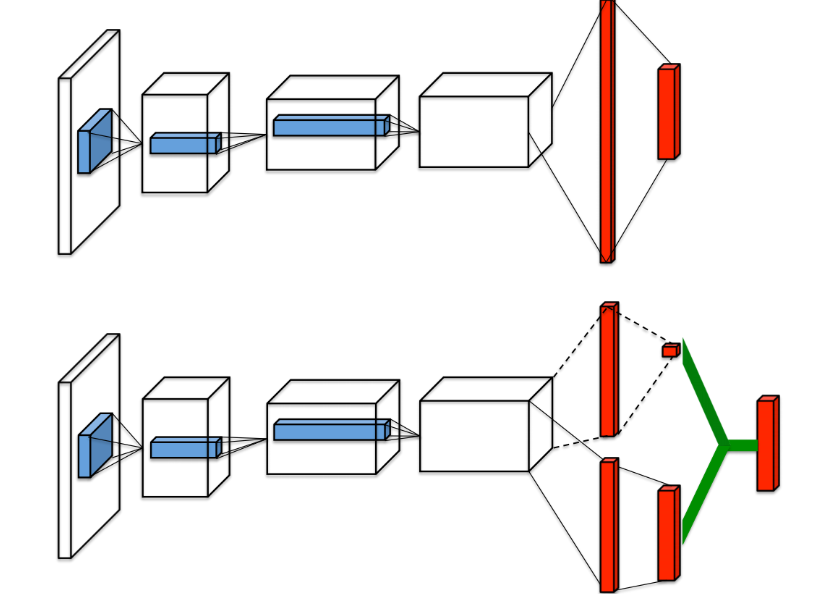
\includegraphics[width=0.5\linewidth]{figures/LiteratureStudy/RL_diagram_Dueling.png}
    \caption{\cite{wang2016dueling}. The top network is a standard Q-network, and the bottom network has a duelling architecture with two separate streams, the value and advantage streams.}
    \label{fig:enter-label}
\end{figure}

\subsubsection{Double Q-learning}
\label{sec:Double_Q_learning}

Standard DQNs tend to be biased towards over-optimistic value estimations due to the same Q-network selecting and evaluating the action. As a result, van Hasselt \cite{vanhasselt2016deep} proposed decoupling the selection and evaluation stages through a \textit{Double Q-network}, this showed to give better estimates and performances in complex environments.

These two Q-networks use the update rule of \autoref{eq:DoubleQLearning} where the leading network, parameters \(\theta\), is updated each iteration for action \(a_{t+1}\) selection, while the target network, parameters \(\theta^{-}\) evaluates these actions. After a set interval, the target network is updated to lower the over-estimation bias.

\begin{equation}
    Q(s_t, a_t; \theta) \leftarrow Q(s_t, a_t; \theta) + \alpha \left[ R(s_t, a_t) + \gamma Q(s_{t+1}, \arg\max_{a_{t+1}} Q(s_{t+1}, a_{t+1}; \theta); \theta^{-}) - Q(s_t, a_t; \theta) \right]
\label{eq:DoubleQLearning}
\end{equation}